% Based on work by Ivan Rudik, who based it on work by Petr Zemek https://blog.petrzemek.net/2016/07/17/latex-template-for-responses-to-referees-reports/

\documentclass[11pt,leqno]{article}

%------------------------------------------%
%                Packages
%------------------------------------------%
 
\usepackage[utf8]{inputenc}
\usepackage{csquotes}
\usepackage{microtype,xparse,tcolorbox}
%These are the packages that we will use in our latex document. 

\usepackage{graphicx}
\usepackage{natbib}	%Bibliography package. It handles citations and can easily change formats. This is done at the end of the document
\usepackage[utf8]{inputenx}% For proper input encoding
\usepackage{adjustbox} %Handles resizing of tables, figures, etc. Based off of page and/or line width/height 
% Packages for tables
\usepackage{booktabs}% For Pretty tables
\usepackage{threeparttable}% For Notes below table
\usepackage{rotating}% To Rotate Table
\usepackage{amsmath, amssymb,mathrsfs} %For using math
\usepackage{bm}
\usepackage{caption} 
\usepackage[list=true]{subcaption} %For having multiple figures within the same one. Figure 1, with part (a) and (b)
%\setcounter{lofdepth}{2}
\usepackage{setspace} %Single, Double Space, etc 
\usepackage[paperwidth=8.5in, paperheight=11in,margin=1in]{geometry} %For controlling the dimensions. Very useful for Posters, etc 
\usepackage{chngpage} 
\usepackage{everypage}%For page numbers on rotated pages
\usepackage[capposition=top]{floatrow}
\usepackage{accents}
\usepackage{float}
\usepackage{comment}
\usepackage{morefloats}
\usepackage{placeins}% To Create Float Barriers so the tables will stay in their sections
\usepackage{pdflscape}

\usepackage{siunitx} %This aligns tables by their decimal and handles processing of the numbers within the tables
  \sisetup{
    detect-mode,
    group-digits      = false,
    input-symbols     = {( ) [ ] - +},
    table-align-text-post = false,
    input-signs             = ,
    %parse-numbers=false,
    %scientific-notation = true,
        %round-mode              = places,
        %round-precision         = 2,
        %input-ignore={,},
    %input-decimal-markers={.},
    %group-separator={,},
        } 
\usepackage{grffile}
\usepackage{soul}
\usepackage{color}
\usepackage{caption}
%\captionsetup[figure]{justification=raggedright,singlelinecheck=off}
\sisetup{separate-uncertainty=true}
\usepackage{mathptmx}
\DeclareCaptionLabelFormat{blank}{}


%------------------------------------------%
%              Custom Commands
%------------------------------------------%
%These are the custom commands that I use in the latex document

\newcommand\iid{i.i.d.} %Makes iid a command
\newcommand\pN{\mathcal{N}} %Makes the natural numbers a command


\setcounter{MaxMatrixCols}{20}

\newtheorem{theorem}{Theorem}%[section]
\newtheorem{lemma}[theorem]{Lemma}
\newtheorem{proposition}[theorem]{Proposition}
\newtheorem{corollary}[theorem]{Corollary}
\newtheorem{assumption}[theorem]{Assumption}
\newenvironment{proof}{\paragraph{Proof:}}{\hfill$\square$ \\} %This fixes the problem with dynamic tables for some reason

%For Page Numbers while rotated
\newlength{\hfoot}
\newlength{\vfoot}
\AddEverypageHook{\ifdim\textwidth=\linewidth\relax
\else\setlength{\hfoot}{-\topmargin}%
\addtolength{\hfoot}{-\headheight}%
\addtolength{\hfoot}{-\headsep}%
\addtolength{\hfoot}{-.5\linewidth}%
\ifodd\value{page}\setlength{\vfoot}{\oddsidemargin}%
\else\setlength{\vfoot}{\evensidemargin}\fi%
\addtolength{\vfoot}{\textheight}%
\addtolength{\vfoot}{\footskip}%
\raisebox{\hfoot}[0pt][0pt]{\rlap{\hspace{\vfoot}\rotatebox[origin=cB]{90}{\thepage}}}\fi}
%http://tex.stackexchange.com/questions/209685/landscape-mode-and-page-numbering

% Add an R in front of tables and figures
\renewcommand{\thetable}{R\arabic{table}}
\renewcommand{\thefigure}{R\arabic{figure}}

%------------------------------------------%
%      Matter Related to Table Creation
%------------------------------------------%
%This helps with custom automatic tables. It uses latex  functions
%http://www.jwe.cc/2012/03/stata-latex-tables-estout/
%http://repec.org/bocode/e/estout/estout.html

% *****************************************************************
% Estout related things
% *****************************************************************
\let\estinput=\input % define a new input command so that we can still flatten the document

\newcommand{\estwide}[3]{
    \vspace{.75ex}{
      \textsymbols% Note the added command here
      \begin{tabular*}
      {\textwidth}{@{\hskip\tabcolsep\extracolsep\fill}l*{#2}{#3}}
      \toprule
      \estinput{#1}
      \bottomrule
      \addlinespace[.75ex]
      \end{tabular*}
      }
    } 

\newcommand{\estauto}[3]{
    \vspace{.75ex}{
      \textsymbols% Note the added command here
      \begin{tabular}{l*{#2}{#3}}
      \toprule
      \estinput{#1}
      \bottomrule
      \addlinespace[.75ex]
      \end{tabular}
      }
    }

% Allow line breaks with \\ in specialcells
\newcommand{\specialcell}[2][c]{%
    \begin{tabular}[#1]{@{}c@{}}#2\end{tabular}
}
\DeclareUnicodeCharacter{00A0}{ }
% *****************************************************************
% Custom subcaptions
% *****************************************************************
% Note/Source/Text after Tables
% The new approach using threeparttables to generate notes that are the exact width of the table.
\newcommand{\Figtext}[1]{%
  \begin{tablenotes}[para,flushleft]
  \hspace{6pt}
  \hangindent=1.75em
  #1
  \end{tablenotes}
  }
\newcommand{\Fignote}[1]{\Figtext{\emph{Note:~}~#1}}
\newcommand{\Figsource}[1]{\Figtext{\emph{Source:~}~#1}}
\newcommand{\Starnote}{\Figtext{* p $<$ 0.1, ** p $<$ 0.05, *** p $<$ 0.01. Robust standard errors in parentheses.}}% Add significance note with \starnote
% If you are using hyper-ref (recommended), this command must go after all 
% other package inclusions (from the hyperref package documentation).
% The purpose of hyperref is to make the PDF created extensively
% cross-referenced.

\newcommand{\sym}[1]{\rlap{#1}} %Allows for fancy stars in tables that also works in beamer

% Create a function that works for the non-linear symbols
\newcommand{\nlsym}[1]{\rlap{\append{}{*}{#1}}} %Allows for fancy stars in tables that also works in beamer

% Character substitution that prints brackets and the minus symbol in text mode. Thanks to David Carlisle
\def\yyy{%
  \bgroup\uccode`\~\expandafter`\string-%
  \uppercase{\egroup\edef~{\noexpand\text{\llap{\textendash}\relax}}}%
  \mathcode\expandafter`\string-"8000 }

\def\xxxl#1{%
\bgroup\uccode`\~\expandafter`\string#1%
\uppercase{\egroup\edef~{\noexpand\text{\noexpand\llap{\string#1}}}}%
\mathcode\expandafter`\string#1"8000 }

\def\xxxr#1{%
\bgroup\uccode`\~\expandafter`\string#1%
\uppercase{\egroup\edef~{\noexpand\text{\noexpand\rlap{\string#1}}}}%
\mathcode\expandafter`\string#1"8000 }

\def\textsymbols{\xxxl[\xxxr]\xxxl(\xxxr)\yyy}


%Protects against odd minus sign errors within the tables
\catcode`_11
\protected\def \c__siunitx_minus_tl {$-$}
\catcode`_ 8 

%-----------Tables-------------%
% This Section is needed to make the tables work with amsmath. But because of the \( being open and having no match, Sublime Text thinks that everything after it (all text) is in math mode and hence changes the text color. This annoys me so the only ``solution'' is to just place this preamble here. It seems to work still. 
\makeatletter 
\edef\originalbmathcode{%
    \noexpand\mathchardef\noexpand\@tempa\the\mathcode`\(\relax} %\)

\def\resetMathstrut@{%
  \setbox\z@\hbox{%
    \originalbmathcode

    \def\@tempb##1"##2##3{\the\textfont"##3\char"}%
    \expandafter\@tempb\meaning\@tempa \relax
  }%
  \ht\Mathstrutbox@\ht\z@ \dp\Mathstrutbox@\dp\z@
}
\makeatother %./tables.tex:25: LaTeX Error: Bad math environment delimiter. [\)]
\usepackage{xparse}

\ExplSyntaxOn
\DeclareExpandableDocumentCommand{\append}{mmm}
 {
  #1\prg_replicate:nn{#3}{#2}
 }
\ExplSyntaxOff

\doublespacing


%------------------------------------------%
%      Title Page Info
%------------------------------------------%
\title{Replies for PAPER NUMBER:\\
 ``TITLE''}
\author{AUTHOR}
\date{\today}
\AtBeginDocument{\maketitle\thispagestyle{empty}\noindent}

\begin{document}




\onehalfspacing


%%%%%%%%%%%%%%%%%%%%%%%%%%%%%%%%%%%%%%%%%%%%%
%%%%%%%%%%%%%%%%%%%%%%%%%%%%%%%%%%%%%%%%%%%%%
\section*{Summary}
%%%%%%%%%%%%%%%%%%%%%%%%%%%%%%%%%%%%%%%%%%%%%
%%%%%%%%%%%%%%%%%%%%%%%%%%%%%%%%%%%%%%%%%%%%%
Summary of main changes 
\begin{enumerate}
  \item First thing     
  
  \item Second thing
  
  \item Third thing
\end{enumerate}

\newpage
%%%%%%%%%%%%%%%%%%%%%%%%%%%%%%%%%%%%%%%%%%%%%
%%%%%%%%%%%%%%%%%%%%%%%%%%%%%%%%%%%%%%%%%%%%%
\section*{Editor}
%%%%%%%%%%%%%%%%%%%%%%%%%%%%%%%%%%%%%%%%%%%%%
%%%%%%%%%%%%%%%%%%%%%%%%%%%%%%%%%%%%%%%%%%%%%
Thank you for your helpful comments and guidance. We describe how we have addressed all of your concerns below. \\
\\
Your comments are below,  \fcolorbox{black}{black!10}{{\ttfamily boxed in with a gray background and different font}}. Our responses are in plain text. Any included text from the new manuscript is \fbox{boxed in with a white background and the} \\
\fbox{same font as this text} with the page number noted at the top of the quoted text. 
Any added comments or other differences from the quoted manuscript text and the text appearing in this report {\color{red} {\ttfamily[appears in brackets with a different font and a red color]}}. \\
\\

%%%%%%%%%%%%%%%%%%%%%%%%%%%%%%%
% Editor 1: Short description of comment
\subsection*{Editor: Comment 1} 
%%%%%%%%%%%%%%%%%%%%%%%%%%%%%%%%

% Exact comment- copied and pasted
\begin{tcolorbox}[left = 1em, top = 1ex, bottom = 1ex, colupper=black, colback=black!10, adjusted title = Editor: Comment 1]
    \setlength\parindent{2em}
	\noindent
	\ttfamily
	
	WORD FOR WORD COPY AND PASTE OF COMMMENT
\end{tcolorbox}

% Response

\paragraph{Short indicator of what the point is (e.g., Event study coefficients are hard to read)} Answer 

\paragraph{Short indicator of what the point is (e.g., Event study should use -1 as reference category)} Answer 

In response we have added the following text to the manuscript (beginning on \hl{page XX}).
    
% Text added to manuscript    
	\begin{tcolorbox}[left = 1em, top = 1ex, bottom = 1ex, colupper=black, colback=white, adjusted title = From page \hl{XX}]
    
       EXACT TEXT FROM MANUSCRIPT
    
        \begin{align}
            y_{it} = &~\beta X + \epsilon_{it} \notag
        \end{align}
        
        We report amazing results in Figure~2. {\color{red} {\ttfamily[Figure~\ref{fig:simple_scatter} in this report.}} \\

        {\color{red} {\ttfamily[text continued on next page]}} \\
    \end{tcolorbox}    
    
    \newpage
    \begin{tcolorbox}[left = 1em, top = 1ex, bottom = 1ex, colupper=black, colback=white, adjusted title = From page \hl{XX} (continued)]
        {\color{red} {\ttfamily[continued from previous page]}}\\
        
        MORE WORDS
        
     
    \end{tcolorbox}
\FloatBarrier
    % Scatter Plot 
\begin{figure}[h]
    \caption[Abbreviated Caption]{A really really really really really really really really really really really really really really really long figure caption to illustrate how you can make a shorter abbreviation in the table of contents.}
      \centering
      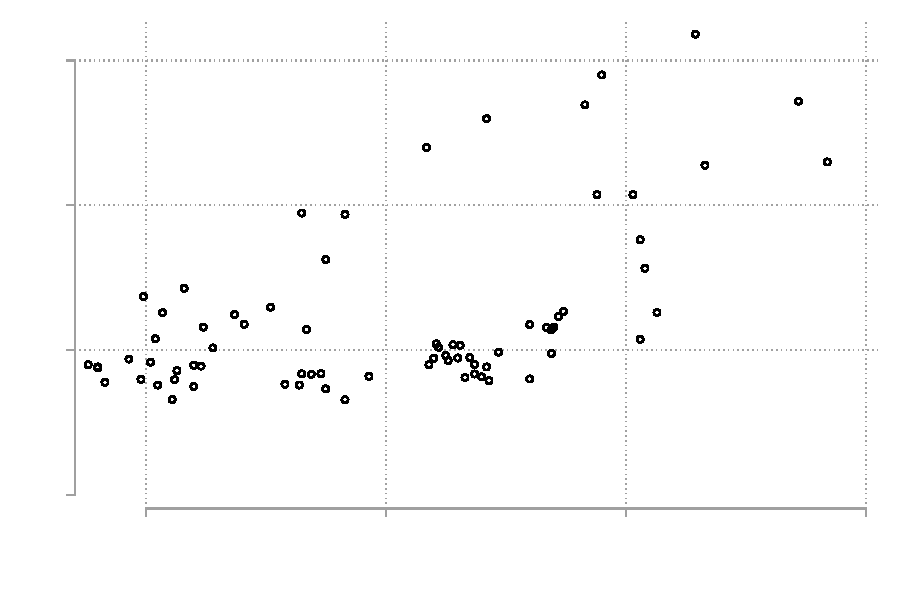
\includegraphics[width=\linewidth]{output/simple_scatter.pdf}

        \subcaption*{\emph{Note:} A very important note.}   
    \label{fig:simple_scatter}
\end{figure}
\FloatBarrier

 \newpage
%%%%%%%%%%%%%%%%%%%%%%%%%%%%%%%%%%%%%%%%%%%%%
%%%%%%%%%%%%%%%%%%%%%%%%%%%%%%%%%%%%%%%%%%%%%
\section*{Referee 1}
%%%%%%%%%%%%%%%%%%%%%%%%%%%%%%%%%%%%%%%%%%%%%
%%%%%%%%%%%%%%%%%%%%%%%%%%%%%%%%%%%%%%%%%%%%%
Thank you for your helpful comments and guidance. We describe how we have addressed all of your concerns below. \\
\\
Your comments are below,  \fcolorbox{black}{black!10}{{\ttfamily boxed in with a gray background and different font}}. Our responses are in plain text. Any included text from the new manuscript is \fbox{boxed in with a white background and the} \\
\fbox{same font as this text} with the page number noted at the top of the quoted text. 
Any added comments or other differences from the quoted manuscript text and the text appearing in this report {\color{red} {\ttfamily[appears in brackets with a different font and a red color]}}. \\
\\

%%%%%%%%%%%%%%%%%%%%%%%%%%%%%%%
% Referee 1: Short description of comment
\subsection*{Referee: Comment 1} 
%%%%%%%%%%%%%%%%%%%%%%%%%%%%%%%%

% Exact comment- copied and pasted
\begin{tcolorbox}[left = 1em, top = 1ex, bottom = 1ex, colupper=black, colback=black!10, adjusted title = Referee: Comment 1]
    \setlength\parindent{2em}
	\noindent
	\ttfamily
	
	WORD FOR WORD COPY AND PASTE OF COMMMENT
\end{tcolorbox}

% Response

\paragraph{Short indicator of what the point is (e.g., Event study coefficients are hard to read)} Answer 

\paragraph{Short indicator of what the point is (e.g., Event study should use -1 as reference category)} Answer 

In response we have added the following text to the manuscript (beginning on \hl{page XX}).
    
% Text added to manuscript    
	\begin{tcolorbox}[left = 1em, top = 1ex, bottom = 1ex, colupper=black, colback=white, adjusted title = From page \hl{XX}]
    
       EXACT TEXT FROM MANUSCRIPT
    
        \begin{align}
            y_{it} = &~\beta X + \epsilon_{it} \notag
        \end{align}
        
        We report all coefficient estimates in Table~2. {\color{red} {\ttfamily[Table~\ref{tab:main_results}in this report.}} \\

        {\color{red} {\ttfamily[text continued on next page]}} \\
    \end{tcolorbox}    

    \newpage    
    \begin{tcolorbox}[left = 1em, top = 1ex, bottom = 1ex, colupper=black, colback=white, adjusted title = From page \hl{XX} (continued)]
        {\color{red} {\ttfamily[continued from previous page]}}\\
        
        MORE WORDS
        
     
    \end{tcolorbox}
\FloatBarrier
    \begin{table}[ht]\centering
            \begin{adjustbox}{width=\textwidth}
            \centering
              \begin{threeparttable}
                \caption{Regression Results}
                \estauto{output/important_table}{5}{S[table-format=1.2,table-column-width=20mm]}
                \label{tab:main_results}
               % \Figtext{Some basic text about the table.}
                \Fignote{* p $<$ 0.1, ** p $<$ 0.05, *** p $<$ 0.01.  Standard errors in parentheses.}              %\Figsource{We good the data from here.}
              % \Starnote
              \end{threeparttable}
             \end{adjustbox}
        \end{table}
\FloatBarrier

\end{document}